\documentclass[11pt]{article}
\usepackage{graphicx} % Required for inserting images
\usepackage{wrapfig}
\usepackage{float}
\usepackage{tabularx}

\usepackage[a4paper,
            left=1in,
            top=1.5in,
            right=1in]{geometry}
\usepackage{hyperref}
\hypersetup{
    colorlinks=true,
    linkcolor=blue,
    filecolor=magenta,      
    urlcolor=cyan,
    pdftitle={Overleaf Example},
    pdfpagemode=FullScreen,
    }

\title{Networked software for distributed systems\\Project 5}
\date{2022-2023}

\begin{document}

\begin{titlepage}
\begin{center}
		\begin{figure}[ht]
			\centering
\includegraphics[width=0.7\textwidth]{resources/Logo_Politecnico_Milano.png}
		\end{figure}
        
        \vspace{3.5cm}

        \LARGE
        \textit{Networked software for distributed systems}\\

        \vspace{0.5cm}
        \Large
        \textbf{Analysis of COVID-19 Data}
        
        \vspace{\fill}
  
		\large
		\begin{tabularx}{\linewidth}{@{}lXl@{}}
			\textit{Authors:}  & & \textit{Professors:} \\
			Stefano Carraro      & & Prof.\@ Luca Mottola\\
			Stefano Fossati  & & Prof. Alessandro Margara \\
			Andrea Restelli & & \\
		\end{tabularx}		
		\thispagestyle{empty}

        \vspace{1cm}

        2022-2023
           
\end{center}
\end{titlepage}

\tableofcontents
\cleardoublepage

%%%
\section{Introduction}
\subsection{Description}
In this project, you have to implement a food delivery application. The application consists of a frontend that accepts requests from users and a backend that processes them. There are three types of users interacting with the service: (1) normal customers register, place orders, and check the status of orders; (2) admins can change the availability of items; (3) delivery men notify successful deliveries. The backend is decomposed in three services, following the microservices paradigm: (1) the users service manages personal data of registered users; (2) the orders service processes and validates orders; (3) the shipping service handles shipping of valid orders. Upon receiving a new order, the order service checks if all requested items are available and, if so, it sends the order to the shipping service. The shipping service checks the address of the user who placed the order and prepares the delivery. 

\subsection{Assumption and Guidelines}
\begin{itemize}
    \item Services do not share state, but only communicate by exchanging messages/events over Kafka topics
    \begin{itemize}
        \item[o] They adopt an event-driven architecture: you can read chapter 5 of the book “Designing Event-Driven Systems” to get some design principles for your project
    \end{itemize}
    \item Services can crash at any time and lose their state
    \begin{itemize}
        \item[o] You need to implement a fault recovery procedure to resume a valid state of the services
    \end{itemize}
    \item You can assume that Kafka topics cannot be lost
    \item You can use any technology to implement the frontend (e.g., simple command-line application or basic REST/Web app)
\end{itemize}

\subsection{Additional Assumption}
\begin{itemize}
    \item We assume that the DB is always available
\end{itemize}
\cleardoublepage

%%%

\section{Design}
\subsection{Microservices communication}
The requirements specify that we have three different microservices that communicate through Kafka. Firstly, we have analyzed the data needed by each microservice in order to efficiently manage the data communication. Secondly, following the suggestions in \href{https://www.confluent.io/designing-event-driven-systems/}{chapter  5 of the book “Designing Event-Driven Systems”}, we have analyzed the entire system and identified which microservice needs to send data (acting as a Kafka producer) and which microservice needs to receive the data (acting as a Kafka consumer).


\paragraph{Communication user service-shipping service:}  
The User Service is responsible for managing user registration and saving user data. This service needs to send data to the Shipping Service in order to communicate the delivery address. Therefore, the User Service must save the user registration in its database and send the data to the Shipping Service through Kafka. We need to ensure that this sequence is atomic. Further details will be explained in the subsequent chapter.

\paragraph{Communication order service-shipping service:}
The Order Service handles user orders and also updates the item availability managed by the admin. This service communicates with the Shipping Service in the following way: first, the Order Service receives the user request; second, the request is validated by checking the availability of items and is then saved in the Order Service database; finally, the Order Service sends the order data to the Shipping Service, which needs to save the data in its own database.

\subsection{Technologies}

For the system design, we have opted to leverage the Spring Boot framework, which offers several advantages:

\begin{itemize}
    \item Seamless integration with databases
    \item Facilitates the setup of REST APIs
    \item Provides convenient access to Kafka APIs
    \item Easy tuning and configuration of Kafka settings
\end{itemize}

However, it's important to note a few drawbacks we have encountered. One such limitation is that Kafka does not support \textbf{XA transactions}. This means that it is unable to group multiple transactions involving different resources into a single reliable global transaction. Consequently, it is not possible to perform an update on a Kafka topic and a database simultaneously within a single transaction. 
This limitation demanded additional effort to identify a suitable workaround.

\subsubsection{Consistency problem}
The fact that Spring does not allow writing to the database and sending data to Kafka within the same transaction can lead to consistency problems.
We will focus only on the communication between the User Service and the Shipping Service, as the communication between the Order Service and the Shipping Service follows a similar pattern, with the only difference being the data processing.
As mentioned in the previous chapter, data is saved in both the User Service and the Shipping Service databases. This design approach introduces data duplication, which can potentially lead to data inconsistency. \\ 
In order to make the data consistent, we have to check that when the user service writes on its database the same data has to be transmitted to the shipping service and that the data is saved in the shipping service database. So each of the following parts need to be atomic:
\begin{itemize}
    \item saving on the producer database (user service)
    \item sending to Kafka topic (user service)
    \item reading from Kafka topic  (shipping service)
    \item saving on the consumer database (shipping service)
\end{itemize}

\paragraph{Producer}

We cannot use a single transaction to write on the database and to send the data to Kafka: so we have two separate steps. We have decided to implement the \href{https://microservices.io/patterns/data/transactional-outbox.html}{transactional outbox pattern} that guarantees to send to Kafka at least one message.

\begin{figure}[H]
    \centering
    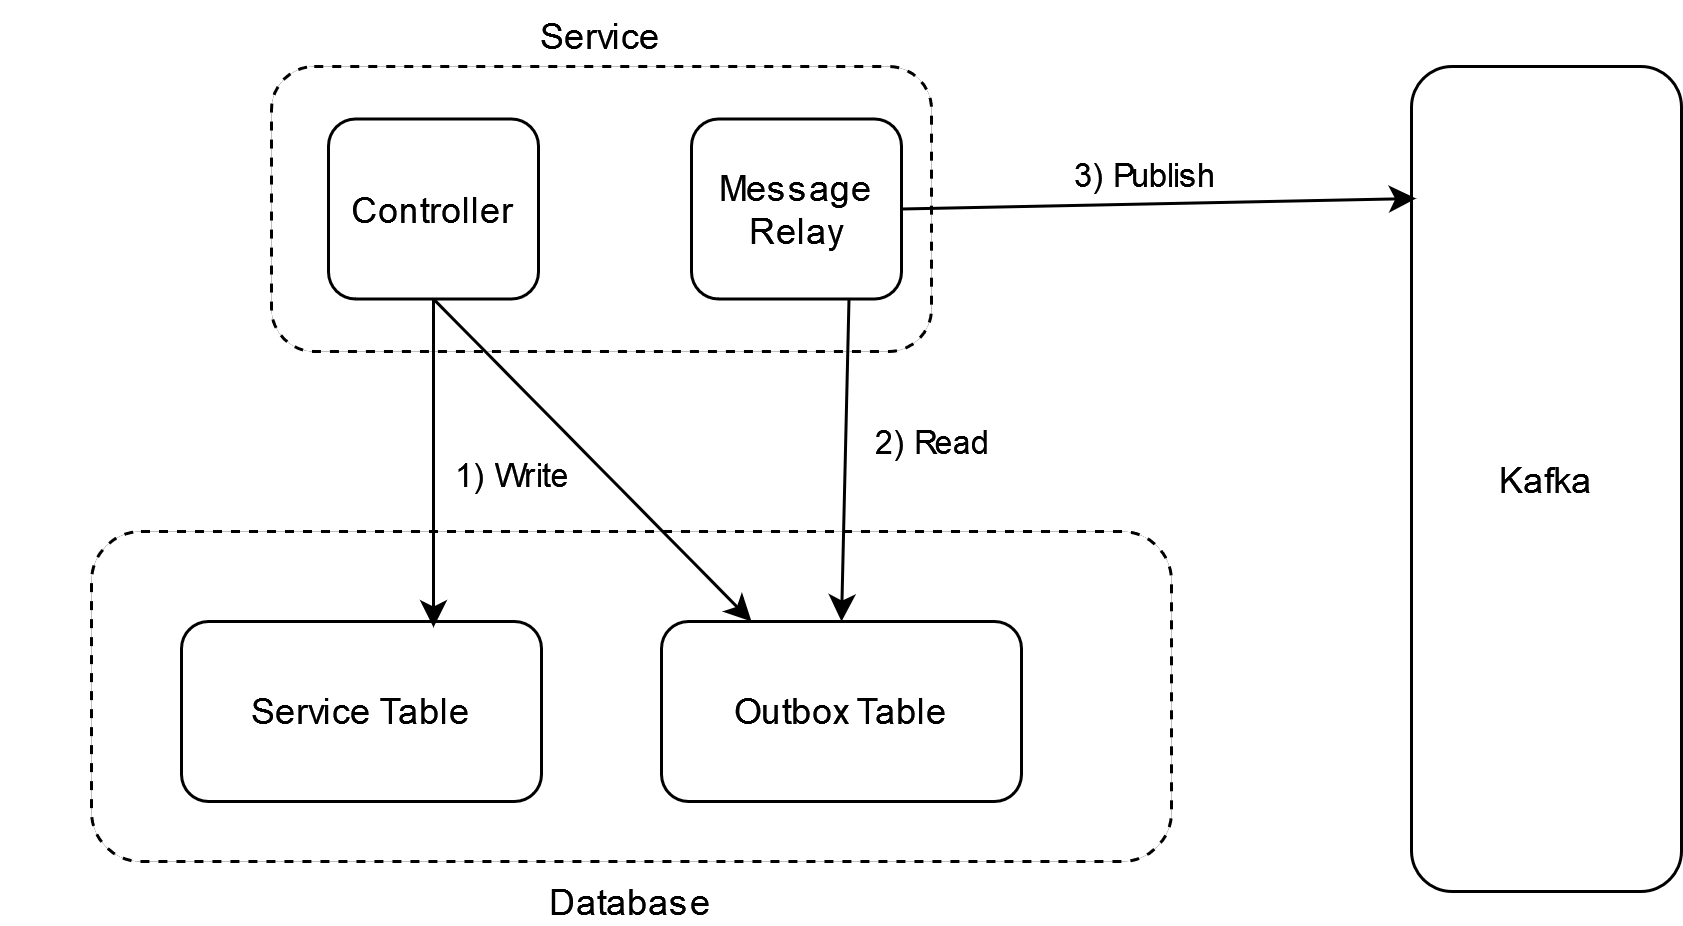
\includegraphics[width=0.7\linewidth]{resources/Trasnactional-outbox-pattern.png}
    \caption{Transactional Outbox pattern schema}
\end{figure}

\begin{itemize}
    \item First, the service needs to save the data in its database. This procedure is performed twice, with the data being stored in two different tables within a single transaction. By executing this as a single transaction, we ensure that either the data is saved in both tables or not saved in either of them, maintaining data consistency.
    \item To achieve a single transaction, the service reads the data from the outbox table and sends it. This approach allows us to send the data in a single operation.
    \item In the final step, the outbox table in the database needs to be modified. The sent data, which was retrieved in the previous step, is deleted from the outbox table, indicating that it has been successfully processed and sent.
\end{itemize}

\paragraph{Consumer}
The consumer is designed to read the latest value of an element from Kafka and save it in the local database. The service consumer performs the following steps within a single transaction:

\begin{itemize}
    \item Read the data from Kafka.
    \item Save the data in the local database.
    \item Commit the offset.
\end{itemize}

Since the consumer is configured to read only the last value, it guarantees that it will read from Kafka exactly once during normal operation. This is achieved by using a unique key for each order when the producer sends the order to Kafka.
\\
To handle the scenario where the consumer reads from Kafka, saves the data in the database, but crashes before committing the offset, a fault tolerance procedure has to be implemented.

\subsubsection{Fault Tolerance}
The fault tolerance procedure is triggered when the consumer service boots up. The procedure involves checking if the first element read from the Kafka topic is already saved in the local service database. 
\begin{itemize}
    \item If the element is found in the database, it indicates that the service previously crashed before committing the offset on the Kafka topic. In this case, the service avoids saving a duplicate entry and proceeds to commit the offset, ensuring that it does not reprocess the same message.
    \item On the other hand, if the element is not present in the database, it signifies that the service crashed before saving it. In this scenario, the service saves the element normally, ensuring data consistency, and then commits the offset on the Kafka topic.
\end{itemize}
By implementing this fault tolerance procedure, the consumer service can recover from potential crashes and resume processing messages from the Kafka topic without duplicating data or missing any messages.

\subsubsection{EOS guarantees}
To ensure Exactly Once Semantics (EOS) in the end-to-end flow of communication between the User Service and Shipping Service, as well as between the Order Service and Shipping Service, we leveraged the guarantees offered by Kafka.
\begin{itemize}
    \item \textbf{Producer side}: we set \textit{enable.idempotence=true} to enforce deduplication of writes on the Kafka topic. This \href{https://developer.confluent.io/patterns/event-processing/idempotent-writer/}{ensures} that duplicate messages are not produced, providing idempotent behavior.
    \item \textbf{Consumer side}: we set \textit{log.cleanup.policy=compact} to \href{https://docs.confluent.io/kafka/design/log_compaction.html#compaction-guarantees}{ensure} that, for each key, only the last value written to the topic is retained. By maintaining a compacted log, we ensure that consumers receive a consistent and up-to-date view of the data, preserving the EOS semantics.
\end{itemize}
These configurations and settings contribute to achieving reliable and consistent message delivery while maintaining the EOS guarantees in the communication flow between microservices.


\section{Implementation and Deployment}
In this section we descibe how we implemented and deployed the services.

\subsection{Implementation}
The implementation of our application adhered to the conventional structure enforced by Spring Boot, with the following organization:

\begin{itemize}
    \item \textbf{Controllers}: where the APIs are exposed, they call business logic methods on the underlying Service layer.
    \item \textbf{Services}: Components where the business logic of the application is implemented. They expose service functions called by Controllers and Consumers and call functions on Repositories to push items on the database and Producers to send events on Kafka topics.
    \item \textbf{Repositories}: DAO components that provide an abstraction layer for interacting with the underlying database.
\end{itemize}

This division allowed for a clear separation of concerns and a structured approach to the application's components.

\begin{figure}[H]
    \centering
    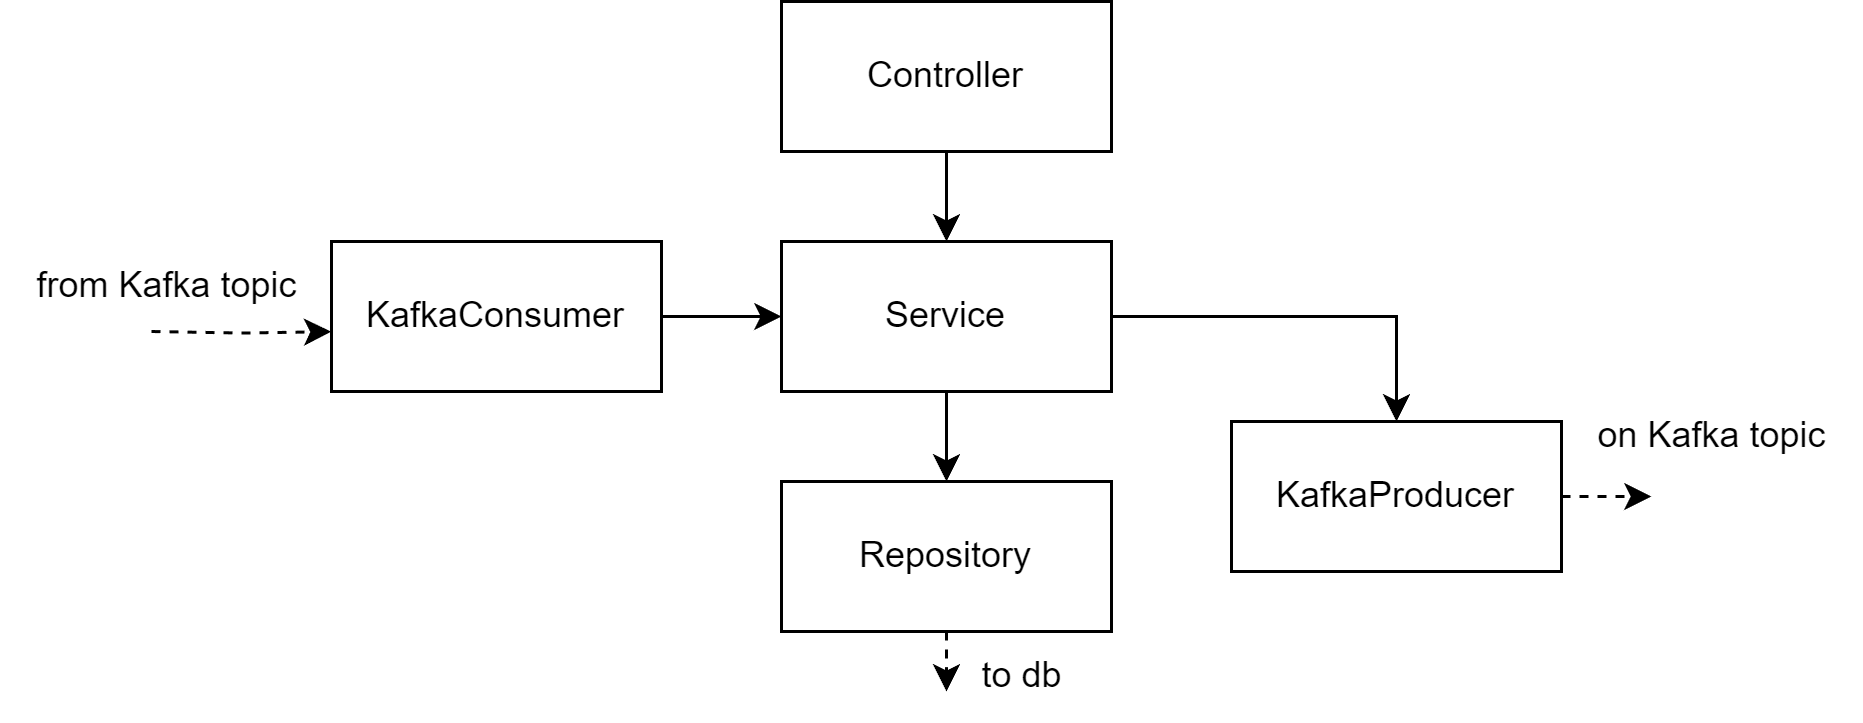
\includegraphics[width=1\linewidth]{resources/Implementation.png} 
    \caption{The interaction between components of the system}
\end{figure}

\subsection{Deployment}

For the deployment of the microservices we exploited Docker. This tool allows us to run each microservice in a single virtualization container, so that each microservice has its own resources.
Also the webserver, the database, Kafka and Zookeeper are running in different containers that expose the APIs.
We have to specify that the database container is a single one, but each microservice used its own non-shared schema in the database. 
In our case the webserver is only hosting the website, the APIs calls to the microservices are performed by the client browser.
\begin{figure}[H]
    \centering
    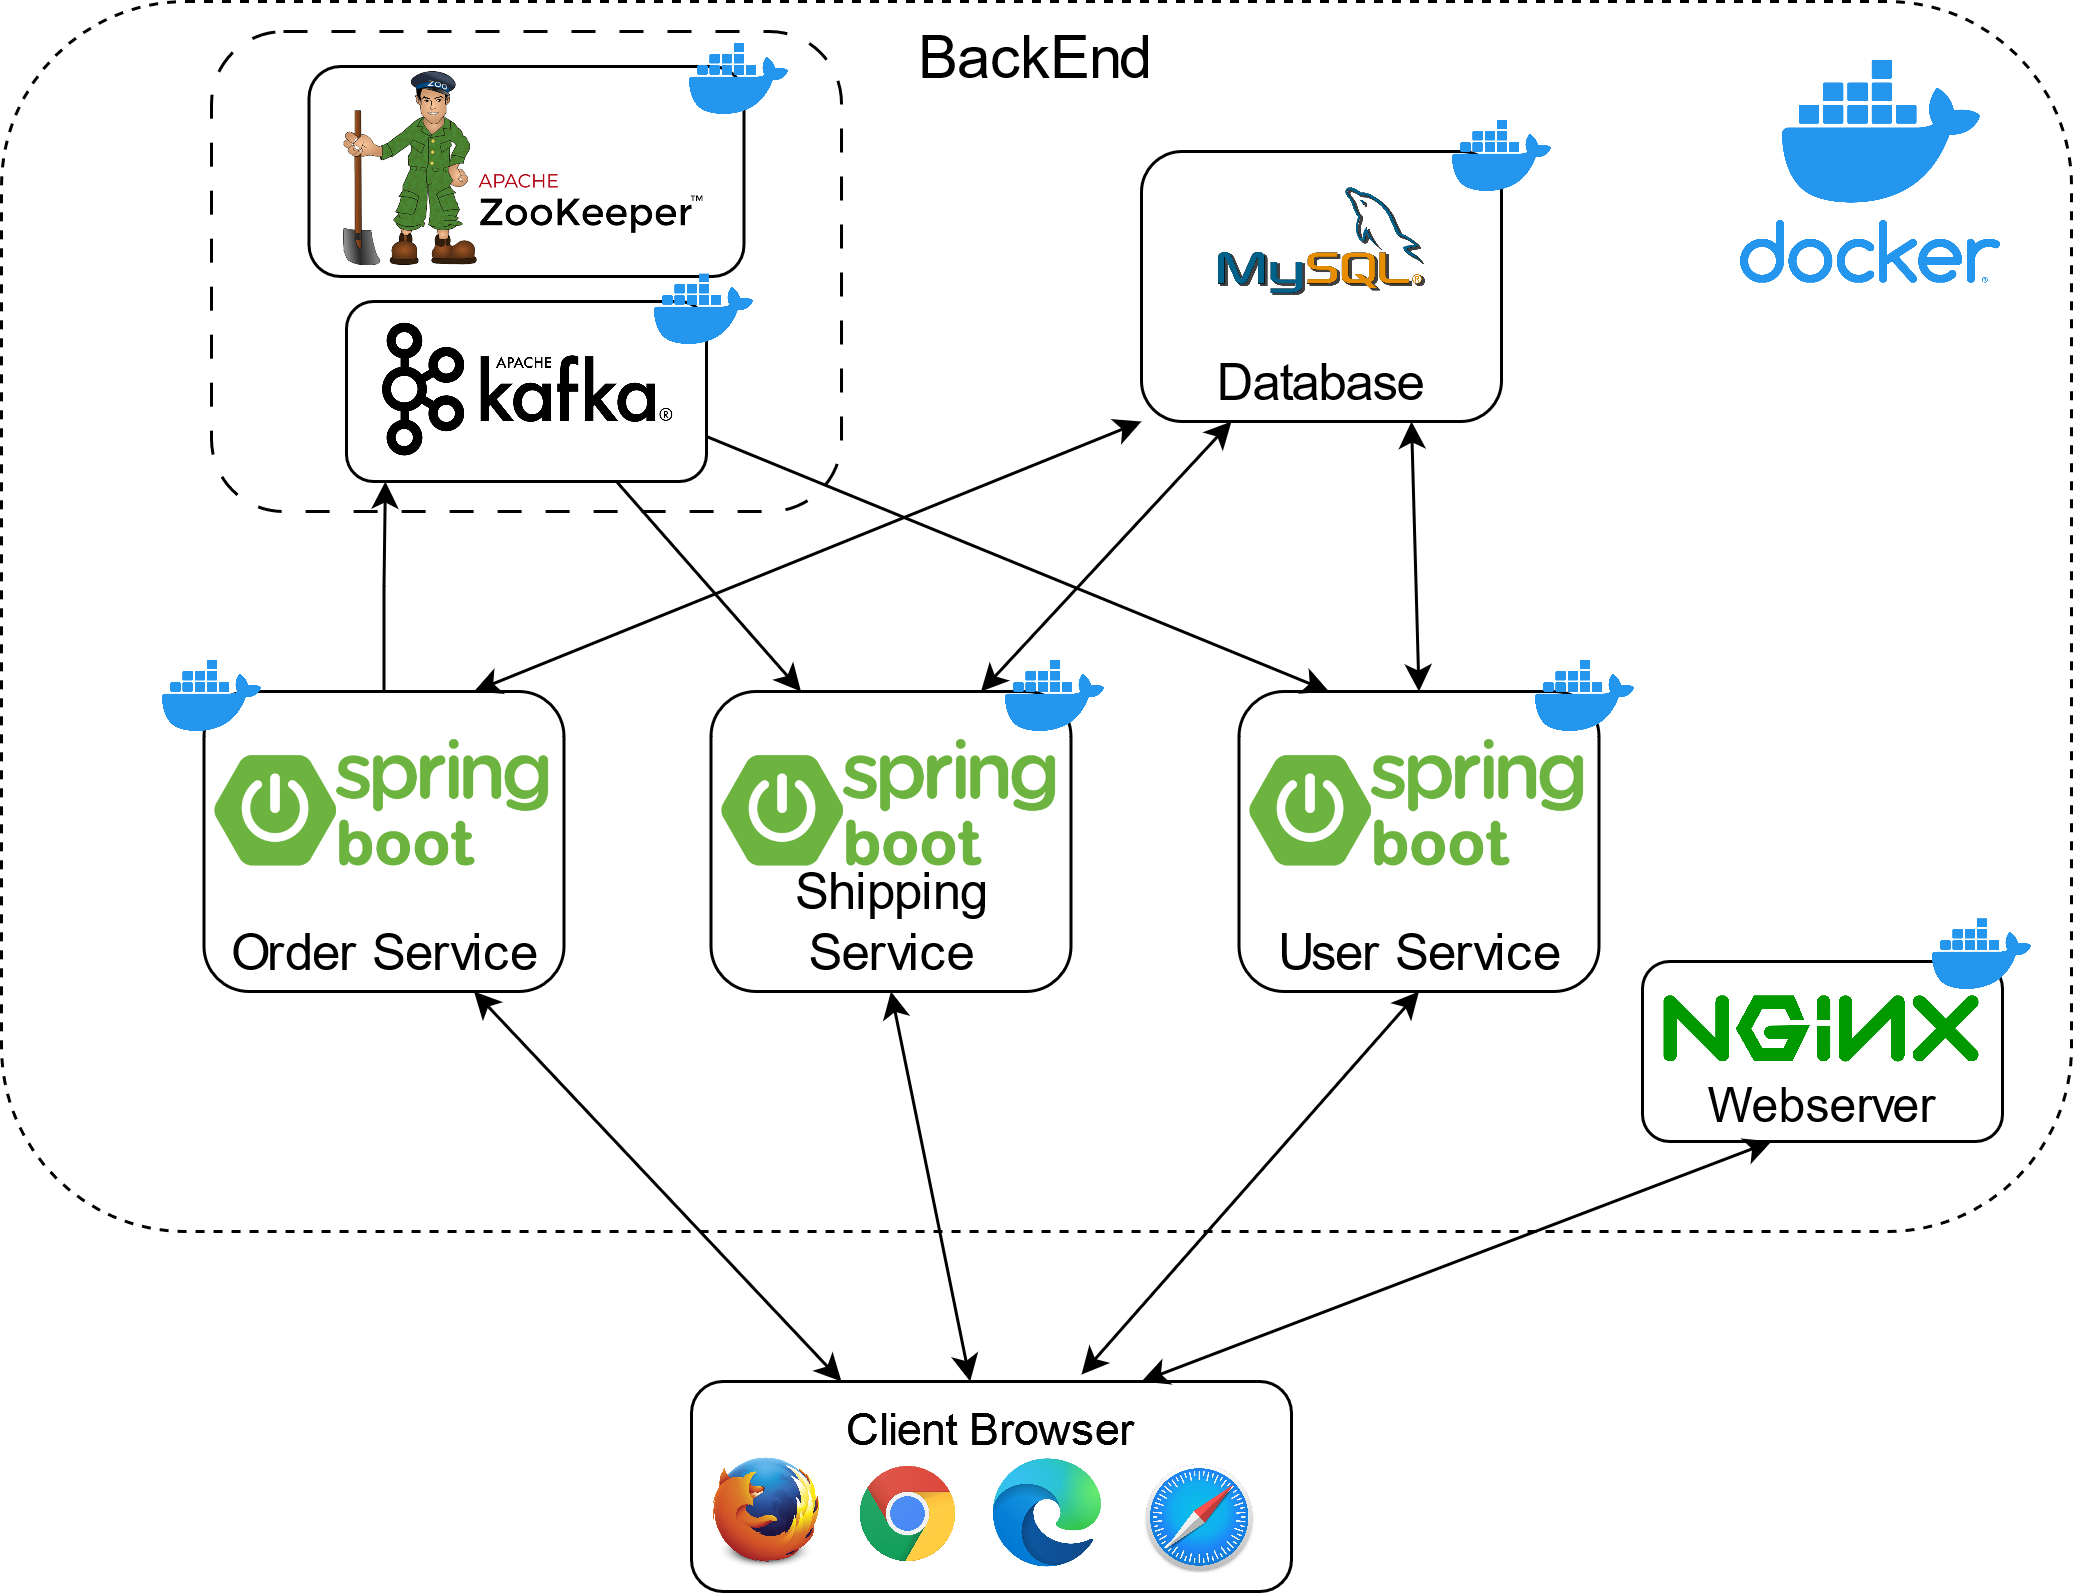
\includegraphics[width=1\linewidth]{resources/Deployment.png} 
    \caption{The deployment structure of the system}
\end{figure}
We decided to use Docker in order to simulate a "real" enterprise environment and also because in this way the project can be tried on every computer that has Docker installed.













\end{document}
